\documentclass{standalone}
\usepackage{graphicx, standalone}
\usepackage[compat=1.1.0]{tikz-feynman}
\usepackage{tikz}
\usepackage{amsmath, amssymb}
\usepackage{euler}
\usepackage{fontspec}
\setmainfont{MinionPro}
\usepackage{comment}

\renewcommand{\k}{\ensuremath\text{k}}
\newcommand{\kp}{\ensuremath\text{k}'}
\newcommand{\q}{\ensuremath\text{q}}
\newcommand{\sing}{\ensuremath\text{s}}
\newcommand{\trip}{\ensuremath\text{t}}

\begin{document}

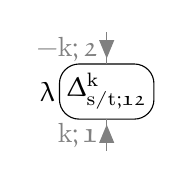
\begin{tikzpicture}[baseline=(current bounding box.center)]
	\begin{feynman}
		\vertex (a);
		\vertex[above=0.4cm of a] (b);
		\vertex[above=0.7cm of b] (c);
		\vertex[above=0.4cm of c] (d);
		\draw[rounded corners=0.25cm] ($(b)+(-0.6,0)$) rectangle ($(c)+(0.6,0)$);
		\vertex at ($(b)+(-0.75,0.35)$) (l) {$\lambda$};
		\node at ($(b)!0.5!(c)$) {$\Delta_{\sing/\trip;\mathfrak{12}}^{\k}$};
		
		\diagram* {
			(a) -- [fermion, gray, edge label=$\k;\mathfrak{1}$] (b),
			(d) -- [fermion, gray, edge label'=$-\k;\mathfrak{2}$] (c)
		};
	\end{feynman}
\end{tikzpicture}
\begin{tikzpicture}[baseline=(current bounding box.center)]
	\node {$=\pm$};
\end{tikzpicture}
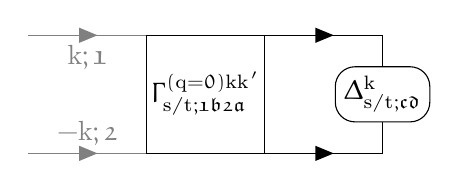
\begin{tikzpicture}[baseline=(current bounding box.center)]
	\begin{feynman}
		\vertex (a1);
		\vertex[below=of a1] (b1);
		\vertex[right=of a1] (a2);
		\vertex[right=of b1] (b2);
		\vertex[right=of a2] (a3);
		\vertex[right=of b2] (b3);
		\vertex[right=of a3] (a4);
		\vertex[right=of b3] (b4);
		
		\vertex[above=0.4cm of b4] (b);
		\vertex[above=0.7cm of b] (c);
		\draw[rounded corners=0.25cm] ($(b)+(-0.6,0)$) rectangle ($(c)+(0.6,0)$);
		\node at ($(b)!0.5!(c)$) {$\Delta_{\sing/\trip;\mathfrak{cd}}^{\k}$};
		\node at ($(b2)!0.5!(a3)$) {$\Gamma_{\sing/\trip;\mathfrak{1b2a}}^{(\q=0)\k\kp}$};
		
		\diagram* {
			(a1) -- [fermion, gray, edge label'=$\k;\mathfrak{1}$] (a2),
			(b1) -- [fermion, gray, edge label=$-\k;\mathfrak{2}$] (b2),
			(b2) -- (b3) -- (a3) -- (a2) -- (b2),
			(b3) -- [fermion] (b4),
			(a3) -- [fermion] (a4),
			(b4) -- (b),
			(c) -- (a4)
		};
	\end{feynman}
\end{tikzpicture}

\end{document}